\documentclass{article}
\usepackage{graphicx} % Required for inserting images
%\usepackage[datesep={}]{datetime2}

\title{Uninvola's Manual v.20240527}
\author{Marco Pezzella}

\usepackage{hyperref}
\usepackage{listings}
\lstset{basicstyle=\ttfamily,
  showstringspaces=false,
  %commentstyle=\color{red},
  %keywordstyle=\color{blue}
}

\newcommand{\uninuvola}{UniNuvola }
\newcommand{\uninuvolan}{UniNuvola}
\newcommand{\jupyterhub}{Jupyterhub }
\newcommand{\jupyterhubn}{Jupyterhub}

\begin{document}
\maketitle
%\part{Introduction}
%\newpage
%\chapter{Introduction}
\part{General instructions}
%\chapter{General usage}
\section{Grant access to \uninuvola}
In order to get access to \uninuvola you will need to have your local account linked to your university identity. This step is done using LDAP. At this stage of the project, this step is done manually by the \uninuvola team. If you need an account, please contact us to the following e-mail:MAIL@UNINUVOLA.\\ 

\section{Connecting to \uninuvola}
\uninuvola can be reached through the \href{uninuvola.fisgeo.unipg.it/}{uninuvola.fisgeo.unipg.it} website, under university network, or using Univerisity of Perugia's VPN. You will be redirect to HPC Vault authenticator page, where you will need to select the "LDAP" option. In the next page, you will required to authenticate with your University credentials. After a correct authentication, you will be directed to the \jupyterhub image selection page (METTI LINK PER SELEZIONE). After choosing your image, you will have access to your space (homepage and storage). \\

\section{Image selection}
After the login, you will invited to select one image to start with. There are 5 available images already compiled with a suite of programs available, and the option of  choosing an external image.  \\

Details on each single image will be discussed in Part\ref{images}, we will briefly introduce the available images:
\begin{itemize}
    \item[\textbf{I}] \textbf{\uninuvola}  \textbf{Base:} Default image of \uninuvola, all other images are based on this one. 
    \item[\textbf{II}] \textbf{Computational Chemistry:} Image containing packages required to perform and analyze chemistry simulations.     
    \item[\textbf{III}] \textbf{Machine Learning:} Image containing packages to perform and analyze various machine learning simulations. 
    \item[\textbf{IV}] \textbf{Computational Physics:} Image containing packages to perform computational fluid dynamics simulations and analysis.
    \item[\textbf{V}] \textbf{Quantum Computing:} Image containing various QC simulators and the libraries for using the SpinQ quantum computer.
\end{itemize}


\begin{figure}[htbp]
    \centering
    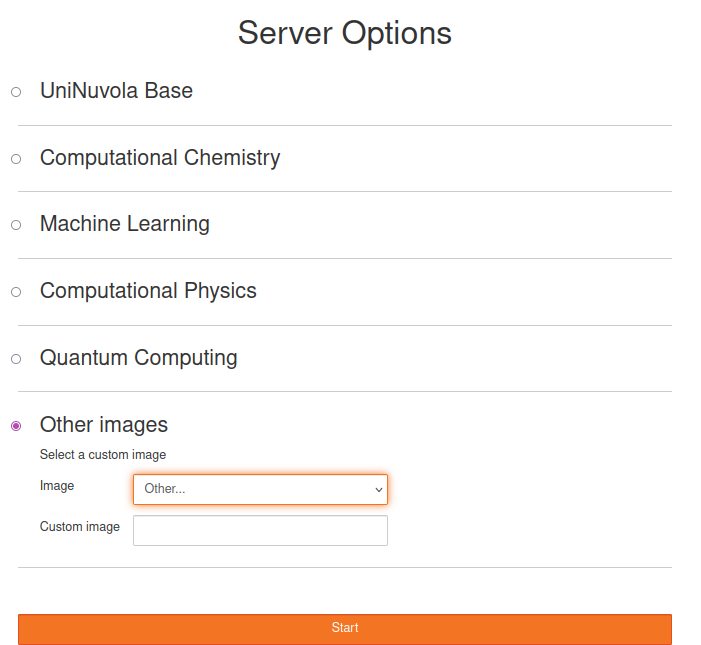
\includegraphics[width=0.75\textwidth]{figures/imageselecton.png}
    \caption{Jupyterhub's image selection page. }
    \label{image_selection}
\end{figure}


\section{Brief description of Jupyterhub}
JupyterHub provides a flexible, scalable, and secure environment for interactive computing. It is a multi-user platform designed for running Jupyter Notebook servers. As a user, you can access individual Jupyter Notebook instances to create and run notebooks, which support multiple programming languages, most commonly Python and R.\\ 

Depending on the future policies of \uninuvola, you will have access to specific computational resources (CPU,GPU,RAM...) allocated to your notebook instance. Your work and data are typically stored persistently, meaning that your files will be saved and available each time you log in.\\

Figure \ref{homepage} shows the homepage for the \uninuvola  ``Default''. The first line of shows all the available notebooks, in this case the classic Jupyter notebook and an Xpra terminal (see Section \ref{xpra}). The default offers a terminal, a general, a Python and Markdown text editors. \\
\begin{figure}[htbp]
    \centering
    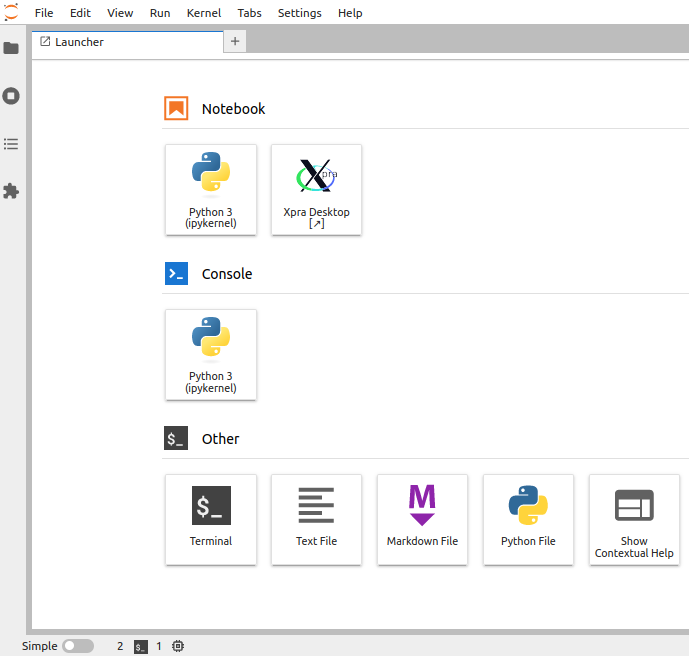
\includegraphics[width=0.75\textwidth]{figures/homepage.png}
    \caption{Homepage of your Jupyterhub home page. }
    \label{homepage}
\end{figure}


\subsection{Xpra}\label{xpra}

Xpra,\cite{Xpra} which stands for "X Persistent Remote Applications," is an innovative open-source tool designed for remote desktop and application forwarding. It allows users to run X11 programs on a remote server while displaying them locally, offering a seamless and flexible remote application experience.\\

With Xpra, you can operate graphical applications on a remote server as if they were running on your local machine, enabling the use of resource-intensive applications on powerful remote servers from a lightweight local client. Another significant advantage of Xpra is session persistence: it allows you to disconnect and later reconnect to your sessions without losing any work. Xpra employs advanced compression techniques and adapts to varying network conditions, ensuring smooth performance even over slower connections. It supports SSH encryption to secure communications between the client and server and can also be configured to use SSL/TLS for additional security. \\

Xpra also facilitates clipboard and audio forwarding, allowing seamless sharing of text or files between local and remote environments and enabling audio streaming from remote applications to your local machine. \\











%\section{Creation of the \textit{.bashrc} file}
%The \textit{.bashrc} file is a powerful tool to customise your Bash environment. It  is a script file %that Bash reads every time it starts a new interactive shell session. It's commonly used to configure %and customise the Bash environment for individual users.  \\ 

%During your first usage of the terminal in \uninuvola, or if you need to recreate your \textit{.bashrc} %file, run the conda initialisation for generating the \textit{.bashrc} file:


%\begin{lstlisting}[language=bash]
%$ bash
%jovyan@jupyter-mp890089$ /opt/conda/bin/conda init
%jovyan@jupyter-mp890089$ source .bashrc
%(base) jovyan@jupyter-mp890089$
%\end{lstlisting}

%This file is used by all the images inside \uninuvola.


\newpage

\part{Available images }\label{images}
%\chapter{Computational Chemistry}
%\usepackage{listings}
%\lstset{basicstyle=\ttfamily,
%  showstringspaces=false,
%  %commentstyle=\color{red},
%  %keywordstyle=\color{blue}
%}


\section{Computational Chemistry}

The following software are included in the Computational Chemistry image:  Ambertools, NAMD3\cite{20PhHaMa}, and two different flavours of DL\_POLY\cite{DLPOLY}: the vanilla version from the CCP5 repository\cite{CCP5}, and DL\_POLY\_ILJ from the University of Perugia. VMD\cite{VMD} is installed as analysis and visualisation tool. \\

\subsection{AmberTools}
AmberTools is installed in a conda environment called \textit{Ambertools}, and it can be used on notebooks or terminals. 

\subsection{DL\_POLY}
DL\_POLY 4 executable is compiled during the image creation process, using the \textit{gfortran} compiler.
The vanilla version is downloaded and compiled from the CCP5\cite{CCP5} Gitlab repository, using the MPI flag and downloading all available tests. The executable, \textit{DLPOLY.Z}, is in the \textit{/usr/bin} directory. \\

A local version of the  DL\_POLY\_ILJ source code (Jan. 2024) is compiled with MPI and \textit{gfortran}. The executable, \textit{DLPOLY\_ILJ.Z}, is in the directory \textit{/usr/bin}. \\

\subsection{NAMD3}
The executable file \textit{namd3} is downloaded from the Urbana University website\cite{NAMD} and is stored in the \textit{/usr/bin} directory.

\subsection{VMD}
The precompiled 1.9.4a55 version of  VMD is installed locally in the image.\cite{VMD,96HuDaSc,98Stxxxx} In order to use the graphical interface, you will need to use the \textit{Xpra Desktop} notebook.

\section{Machine Learning}

The ``Machine Learning'' image contains the libraries for running various marchine learning codes and libraries.  There are two kernels implememented, having tensorflow and pytorch%\chapter{Quantum Computing}
%\usepackage{listings}
%\lstset{basicstyle=\ttfamily,
%  showstringspaces=false,
%  %commentstyle=\color{red},
%  %keywordstyle=\color{blue}
%}
\section{Quantum Computing}
In this chapter we will discuss how to use the  Quantum computer image in \uninuvola. The image contains various quantum computer simulators and the libraries required to run calculations with the SpinQ Triangulum quantum computer remotely. \\ 

\subsection{Python Environments}

\subsubsection{spinqit}
The environment \textit{spinqit} contains all the necessary libraries for running calculations with the \href{https://github.com/SpinQTech/SpinQit}{SpinQit package}. The environment's kernel is Python 3.9.12, as required. The additional pytorch library is included in this library. \\

\subsubsection{ocean}
The environment \textit{ocean} allows the utilisation of the  \href{https://docs.ocean.dwavesys.com/en/stable/}{D-Wave Ocean} library package. 

\subsubsection{qiskit}
The environment \textit{qiskit}, from \href{https://www.ibm.com/quantum/qiskit}{IBM} contains the libraries qiskit, qiskit-aer, qiskit\_ibm\_runtime. 




\section{Using your custom image}
\uninuvola offers the opportunity to load and use your custom image into the server. In this way you can import images from other services and test your own image while building it ( you can find a brief guide on how compile your own image in Section \ref{image_creation}). \\

In  the image selection page, Figure  \ref{image_selection}, you can select the option \textit{Other images} and select \textit{Other}. You will need to type the docker image name in the \textit{Custom image} section using the following formalism: \textit{image\_name:version}. 

\subsection{Example: Pangeo Notebook}
As an example of customised notebook we will import the Pangeo notebook. Pangeo is a community promoting open, reproducible, and scalable Big Data geoscience. Figure \ref{img:pangeo} shows a snippet of the \href{https://hub.docker.com/r/pangeo/pangeo-notebook/tags}{Dockerhub project page}:the page's  title corresponds to the \textit{image\_name}, with each available tag shown in boxes. These information can be found on the right side of each box. 

\begin{figure}[htbp]
    \centering
    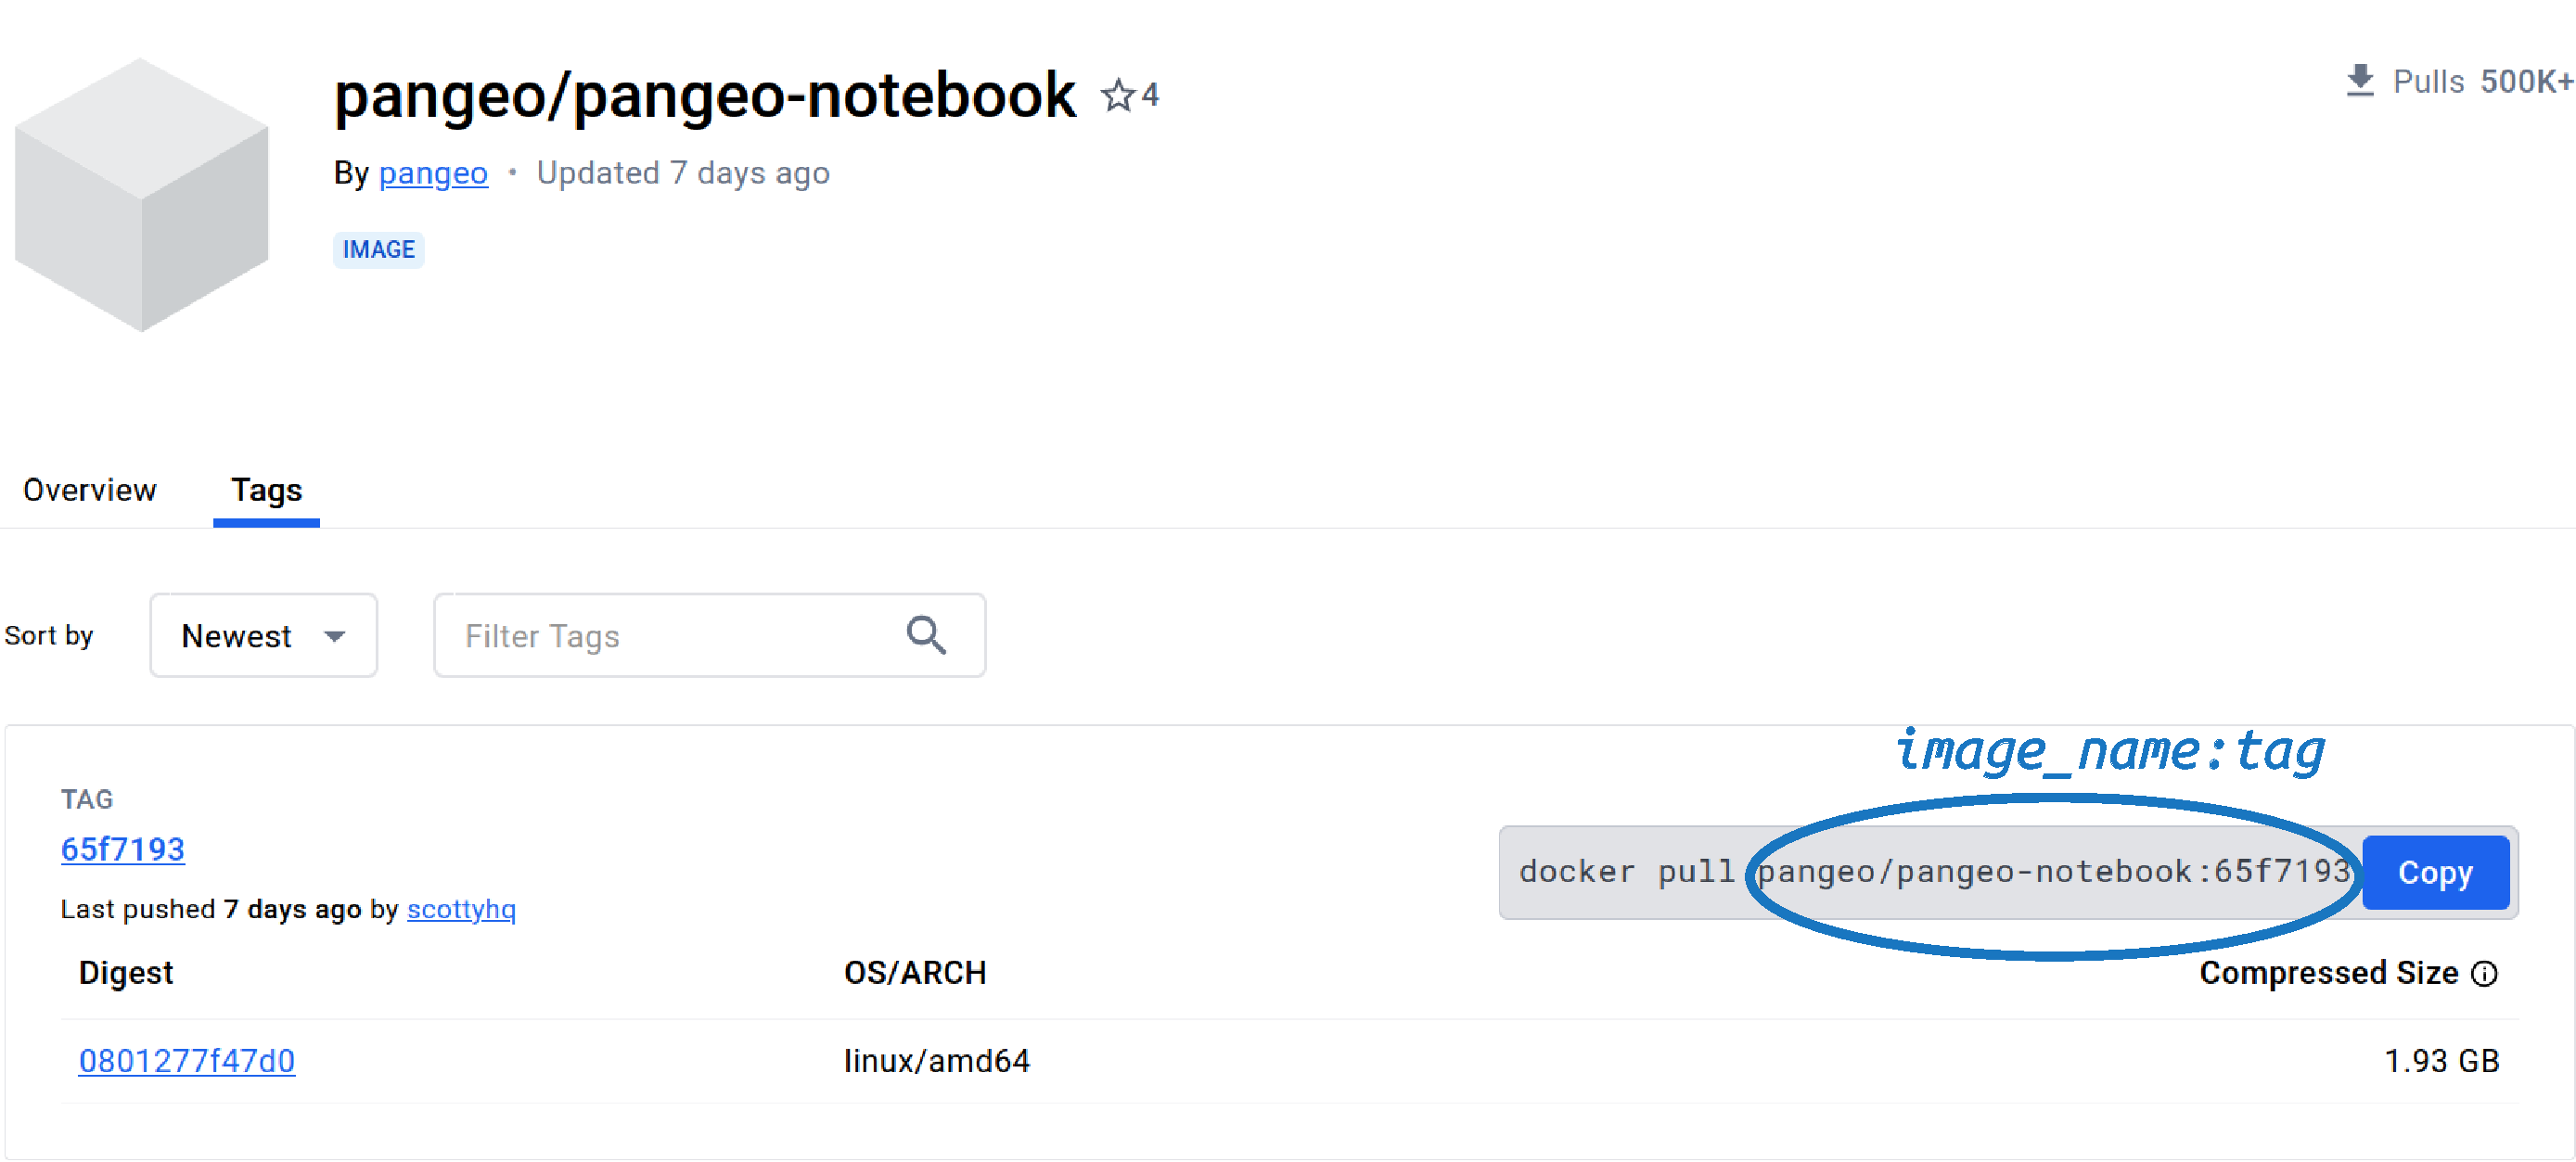
\includegraphics[width=0.9\textwidth]{figures/pangeo.pdf}
    \caption{Dockerhub page for the \href{https://hub.docker.com/r/pangeo/pangeo-notebook/tags}{Pangeo project}. }
    \label{img:pangeo}
\end{figure}

These information are inputted into the custom image cell, as it seen in Figure \ref{img:pangeo_opne}.

\begin{figure}[htbp]
    \centering
    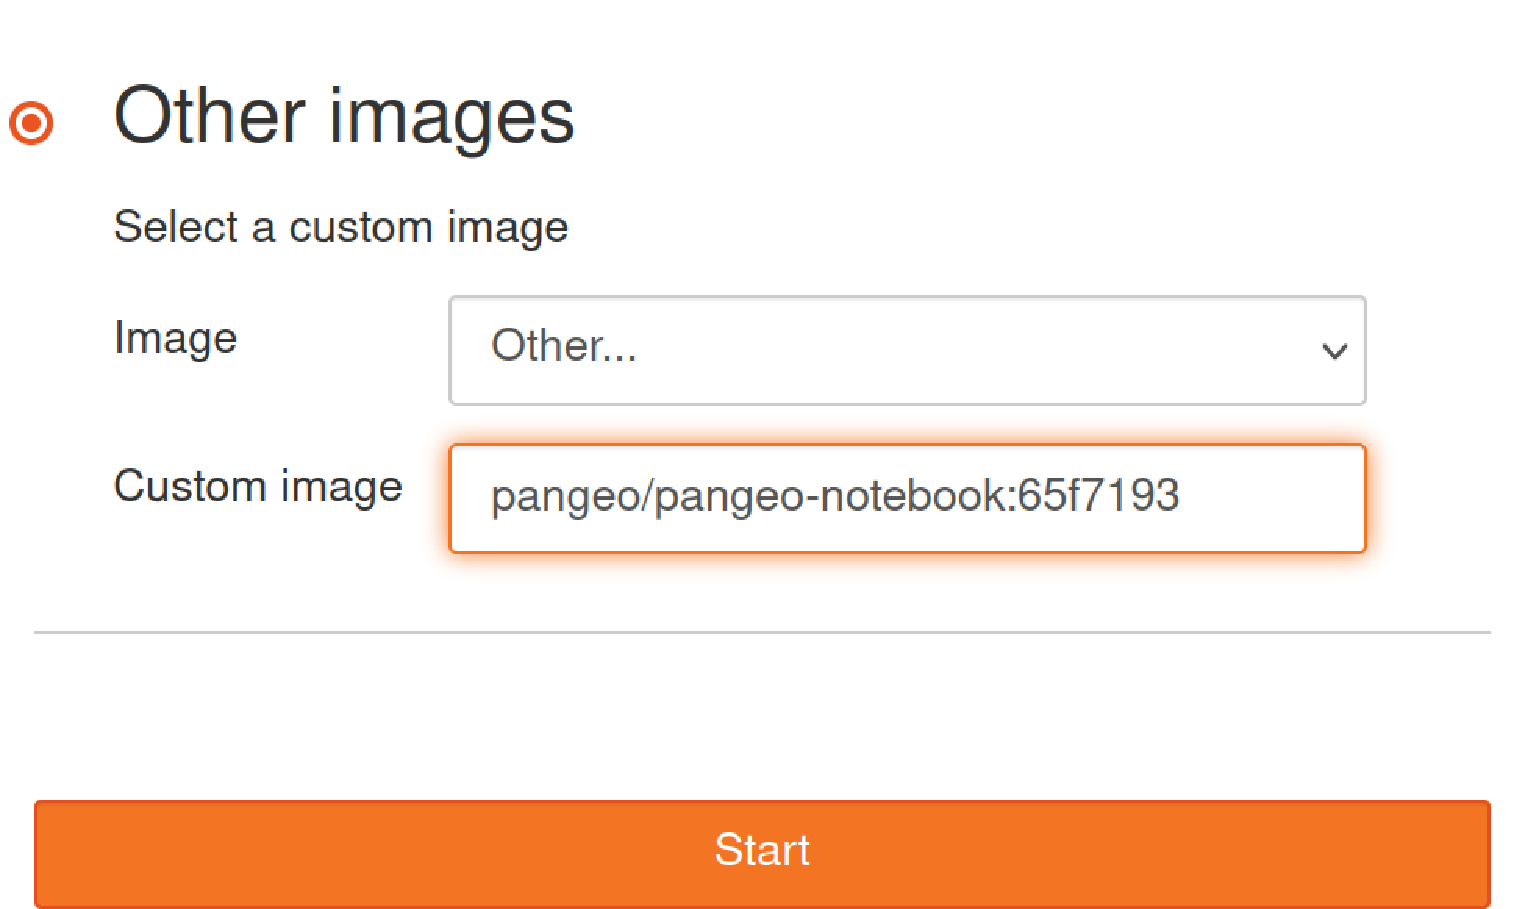
\includegraphics[width=0.75\textwidth]{figures/pangeo_open.pdf}
    \caption{Practical example of custom image selection. }
    \label{img:pangeo_opne}
\end{figure}


%[]


% DA QUELLO CHE VEDO POSSIAMO CARICARE IMMAGINI SOLO DA DOCKERHUB, CHE POTREBBE ESSERE UN PROBLEMA(?). iMMAGINI DA QUAY.IO NON SONO CARICATE. ALTRA COSA DA CONTROLLARE: L'IMMAGINE DEVE ESSERE BASATA SU JHUB GIUSTO? I DOCKER DI FEDORA E R NON PAIONO LAVORARE  
\newpage

\part{Appendices}
%\chapter{Image Creation}
\section{Creation of an image}
All \uninuvola's Docker images are built on top of the ``Default'' image. You can copy one of the available  Dockerfile in your project directory and start modifying it. You can install new packages using the appropriate package managers, using the \textit{RUN} keyword in the Dockerfile

\begin{lstlisting}[language=python]
  RUN apt-get update && apt-get install -y package\_name
\end{lstlisting}

Copy your application code into the Docker image, using the \textit{COPY} (for local files) or \textit{ADD} (for local and remote files) command in the Dockerfile. Do not use the /home directory as the target directory as it will be overwritten when loading the external storage.

\begin{lstlisting}[language=python]
  COPY myfile.txt  /app
  ADD https://example.com/path/to/remote/file.txt /app/
\end{lstlisting}
%5. Set Environment Variables (if needed):
%    If your application relies on environment variables, set them using the ENV keyword in your Dockerfile. For example:
%    ENV ENV_VARIABLE=value

In order to build your Docker Imaga, open a terminal and navigate to the directory containing the Dockerfile. Run the following command to build your Docker image:

\begin{lstlisting}[language=python]
    docker build -f image\_name -t image\_tag .
\end{lstlisting}

The \textit{-f} tag allows you to name your dockerfile with a custom name, while the \textit{-t}  flag allows the user to define a customised tag for your image. Replace image\_name with a suitable name for your Docker image. \\

Once the image is built successfully, you can run a Docker container using the following command:

\begin{lstlisting}[language=python]
    docker run -it image\_tagname 
\end{lstlisting}
    
The \textit{-it} tag allows you to test your image locally and interactively. \\

You can include a .dockerignore file to specify files and directories that should not be copied into the Docker image. 
\section{Quantum computer's calculation example}
The following lines of codes need to be added in your Python script in order to connect to the Triangulum Quantum Computer:

\begin{lstlisting}[language=bash]
username="Ulysses"
password="Odissey"
config.configure_ip("spinq.fisgeo.unipg.it")
config.configure_port(55444)
config.configure_account(username, password)
...
\end{lstlisting}

\noindent  The web address  \textit{spinq.fisgeo.unipg.it} points to the workstation's IP address connected to the Triangulum through the port 55444. \\

\noindent You need to ask your system administrator to create an \textit{username} and \textit{password} in the quantum computer.  
Due to some translation error in the interface, it is advisable to use the same entries for \textit{Account} and \textit{Name} while creating your local account. The variable  \textit{username} corresponds to the entry \textit{Account}.

\subsection{Example: GHZ state}
\begin{lstlisting}[language=bash]
from spinqit import get_nmr, get_compiler, Circuit, NMRConfig
from spinqit import H, CX

username="Ulysses"
password="Odissey"

engine = get_nmr()
comp = get_compiler("native")

circ = Circuit()

q = circ.allocateQubits(3)
circ << (H, q[0])
circ << (CX, (q[0], q[1]))
circ << (CX, (q[1], q[2]))

exe = comp.compile(circ, 0)
config = NMRConfig()
config.configure_shots(1)
config.configure_ip("spinq.fisgeo.unipg.it")
config.configure_port(55444)
config.configure_account(username, password)
config.configure_task("task1", "GHZ")


result = engine.execute(exe, config)
print(result.probabilities)
\end{lstlisting}


\part{Bibliography}
% Choose a bibliography style
\bibliographystyle{plain}
% Specify the .bib file
\bibliography{uninuvola}
\bibliographystyle{plain} 
\end{document}

